% Бүлэг 3
\chapter{Төслийн хэсэг} % Бүлгийн нэр
\label{Chapter3} % Энэ бүлэг рүү ишлэл хийх бол \ref{Chapter1} командыг ашигла 

%-----------------------------------------------------------------------
\section{Өгөгдлийн ерөнхий схем}

\subsubsection{Өгөгдлийн ерөнхий схем}
\begin{figure}[H]
    \centering
    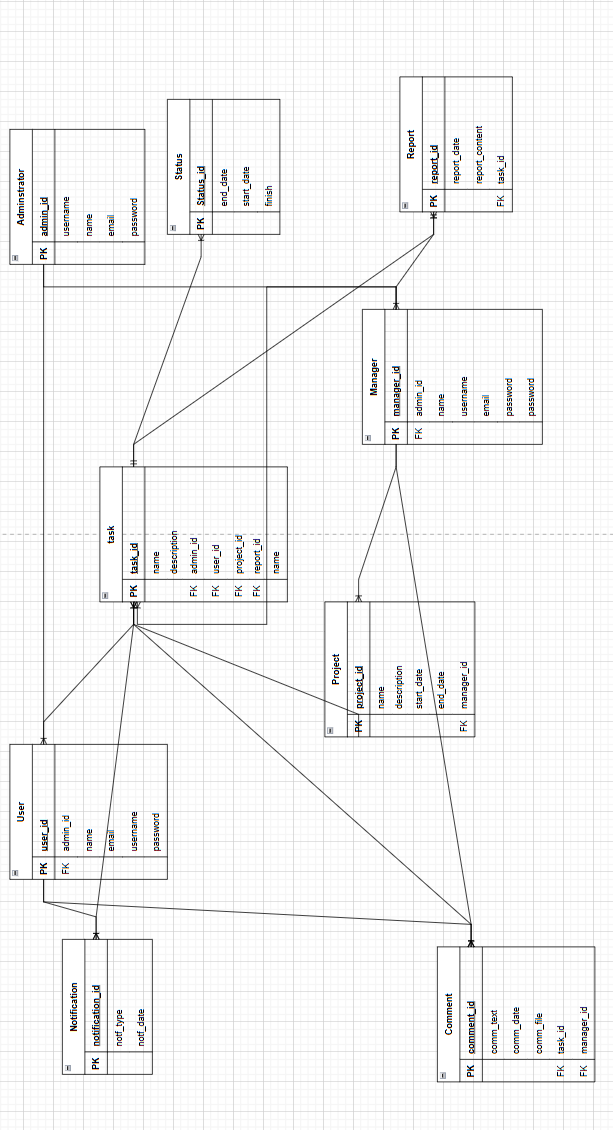
\includegraphics[width=10cm]{Diagrams/erd_diagramm1.PNG} % Зураг байрлал оруулах
    \caption[Өгөгдлийн ерөнхий схем]{Өгөгдлийн ерөнхий схем}
    \label{fig:general_data_schema}
\end{figure}

Классууд

\begin{itemize}
\item \textbf{Хэрэглэгч:} Системд нэвтэрч ашиглах эрх бүхий ерөнхий хэрэглэгчид.
\item \textbf{Админ:} Системийн бүх үйл ажиллагааг хянаж, удирддаг хэрэглэгч.
\item \textbf{Менежер:} Эмийн сангийн үйл ажиллагаа болон бараа материалын менежментийг хариуцдаг хэрэглэгч.
\item \textbf{Эм:} Эмийн мэдээллийг бүртгэх үндсэн объект. Үүнд эмийн нэр, төрөл, үйлдвэрлэсэн огноо, хүчинтэй хугацаа, агуулахад байгаа тоо хэмжээ зэрэг атрибутууд орно.
\item \textbf{Захиалга / Борлуулалт:} Эмийн худалдан авалт, захиалгын мэдээллийг удирдах объект.
\item \textbf{Нийлүүлэлт:} Эм нийлүүлэгчээс ирж буй бараа материалын мэдээлэл.
\item \textbf{Тайлан:} Системийн үйл ажиллагааны дүн шинжилгээ, борлуулалт, үлдэгдэл гэх мэт мэдээллийг харуулна.
\item \textbf{Сэтгэгдэл:} Хэрэглэгчийн санал, зөвлөмжийг бүртгэх объект.
\item \textbf{Мэдэгдэл:} Системээс хэрэглэгчдэд илгээж буй автомат мэдээлэл, сануулга.
\item \textbf{Статус:} Эм, захиалга, нийлүүлэлт болон бусад үйл явцын төлөвийг тодорхойлдог.
\end{itemize}

\section*{Харилцаа холбоо}

\begin{itemize}
    \item Хэрэглэгчид эмийн мэдээллийг харах, захиалга хийх, мөн системээс мэдэгдэл хүлээн авах боломжтой.
    \item Менежерүүд эмийн нөөц, нийлүүлэлт болон захиалгыг хянаж, тайлан гаргах үүрэгтэй.
    \item Эм, захиалга, нийлүүлэлт, тайлан зэрэг объектууд нь хэрэглэгч, менежер, статустай холбогддог.
\end{itemize}



%-----------------------------------------------------------------------
%-----------------------------------------------------------------------
\section{Үйл ажиллагааны диаграм}

Эмийн бүртгэлийн систем нь эмийн мэдээллийг цахим хэлбэрээр бүртгэх, удирдах, хянах зорилготой програм хангамжийн шийдэл юм. Энэхүү систем нь эмийн нэр, төрөл, үйлдвэрлэсэн огноо, хүчинтэй хугацаа, агуулахад байгаа тоо хэмжээ зэрэг мэдээллийг төвлөрсөн байдлаар хадгалах боломжийг олгодог. Доорх хэсэгт системийн үндсэн хэрэглэгчдийн үйл ажиллагааны диаграмыг тус тусад нь үзүүлэв.

\subsubsection{Админы үйл ажиллагааны диаграм}
\begin{figure}[H]
    \centering
    \includegraphics[width=10cm, height=12cm]{Diagrams/admin_activity1.PNG}
    \caption[Админы үйл ажиллагааны диаграм]{Админы үйл ажиллагааны диаграм}
\end{figure}
\begin{itemize}
    \item \textbf{Админ:} Системд нэвтрэх, хэрэглэгчийн бүртгэл үүсгэх, хэрэглэгчийн эрх болон хандалтыг удирдах, системийн ерөнхий тохиргоог хийх, мэдэгдэл илгээх, системийн үйл ажиллагаанд хяналт тавих.
\end{itemize}

\subsubsection{Менежерийн үйл ажиллагааны диаграм}
\begin{figure}[H]
    \centering
    \includegraphics[width=16cm, height=20cm]{Diagrams/manager_activity1.PNG}
    \caption[Менежерийн үйл ажиллагааны диаграм]{Менежерийн үйл ажиллагааны диаграм}
\end{figure}
\begin{itemize}
    \item \textbf{Менежер:} Эмийн мэдээлэл бүртгэх, засварлах, устгах, эмийн нөөц хянах, нийлүүлэлтийг бүртгэх, захиалга болон борлуулалтыг хянах, тайлан гаргах, эмийн үлдэгдэл болон хугацаа дуусах дөхсөн эмүүдийг хянах.
\end{itemize}

\subsubsection{Хэрэглэгчийн үйл ажиллагааны диаграм}
\begin{figure}[H]
    \centering
    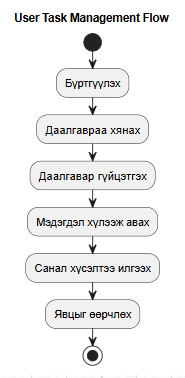
\includegraphics[width=10cm, height=12cm]{Diagrams/user_activity.PNG}
    \caption[Хэрэглэгчийн үйл ажиллагааны диаграм]{Хэрэглэгчийн үйл ажиллагааны диаграм}
\end{figure}
\begin{itemize}
    \item \textbf{Хэрэглэгч:} Системд нэвтрэх, эмийн мэдээлэл харах, эм захиалах, захиалгын төлөв шалгах, санал хүсэлт илгээх, мэдэгдэл хүлээн авах, системээс гарах.
\end{itemize}


\section{Класс диаграм}
\begin{figure}[H]
    	\centering
    \includegraphics[width=16cm]{Diagrams/class_diagram1.PNG}
    	\caption[Класс диаграм]{Класс диаграм}
\end{figure}
\begin{itemize}
    \item \textbf{Администратор:} Хэрэглэгчид болон хандалтыг удирддаг.
    \item \textbf{Менежер:} Төсөл боловсруулж, даалгавар өгч, тайлан гаргадаг.
    \item \textbf{Ажилтан:} Даалгавраа гүйцэтгэдэг.
\end{itemize}
%-----------------------------------------------------------------------
\section{Дарааллын диаграм}
\subsubsection{Эмийн захиалга хийх дарааллын диаграм}

\begin{figure}[H]
    \centering
    \includegraphics[width=16cm]{Diagrams/order_seq.PNG} % <-- зургийнхаа нэрийг энд тааруулна
    \caption[Эмийн захиалгын дарааллын диаграм]{Эмийн захиалгыг хүргэлттэй болон салбараас авах хоёр хувилбараар гүйцэтгэх дарааллын диаграм}
\end{figure}

\begin{itemize}
    \item \textbf{Өвчтөн:}
    \begin{itemize}
        \item Утасгаар эсвэл онлайнаар эмийн \textbf{захиалга өгнө}.
        \item Эмийн сангийн бүртгэгчээс захиалгын мэдээлэл баталгаажсаны дараа хүргэлтээр авах уу, салбараас очиж авах уу гэдгээ сонгоно.
    \end{itemize}

    \item \textbf{Эмийн сангийн бүртгэгч:}
    \begin{itemize}
        \item Өвчтөнөөс ирсэн захиалгыг \textbf{Эмийн захиалга} системд \textbf{бүртгэнэ}.
        \item Захиалагдсан эмийг жагсаалтаас сонгох үйлдлийг давтан (\textit{loop}) хийж, нийт дүнг тооцоолно.
        \item Нийт дүн 40\,000 төгрөгөөс дээш бол 20\% хөнгөлөлтийг системд тооцоолуулна.
        \item Бэлтгэсэн баримтыг өвчтөнд танилцуулж, хүргэлтээр авах эсвэл салбараас авах сонголтыг авна.
    \end{itemize}

    \item \textbf{Эмийн захиалга (систем):}
    \begin{itemize}
        \item Эмийн сангийн бүртгэгчээс ирсэн мэдээлэл дээр үндэслэн захиалга үүсгэж хадгална.
        \item Захиалгад орсон эм бүрийн мэдээллийг \textbf{Эм} объекттой холбон авч, үлдэгдэл болон үнэд суурилан нийт дүнг гаргана.
        \item Хүргэлттэй захиалгын үед хүргэлтийн ажилтанд, салбараас авах захиалгын үед салбарын мэдээлэлд дамжуулна.
    \end{itemize}

    \item \textbf{Эм:}
    \begin{itemize}
        \item Эмийн нэр, төрөл, үнэ, үлдэгдэл зэрэг мэдээллийг \textbf{Эмийн захиалга} системд нийлүүлж, захиалгын үед шалгах үндсэн өгөгдөл болдог.
    \end{itemize}

    \item \textbf{Хүргэлтийн ажилтан ( Хүргэлттэй захиалга):}
    \begin{itemize}
        \item Эмийн сангийн бүртгэгчээс \textbf{“захиалгыг хүргэх хүсэлт”}-ийг хүлээн авна.
        \item Захиалгыг өвчтөнд хүргэж өгөөд, захиалгыг хүлээн авсан тухайгаа системд илгээнэ.
        \item Өвчтөнөөс бэлэн мөнгө эсвэл картын \textbf{төлбөрийг авна}.
    \end{itemize}

    \item \textbf{Төлбөрийн систем:}
    \begin{itemize}
        \item Хүргэлтийн ажилтан эсвэл салбар дээрээс ирсэн төлбөрийн мэдээллийг хүлээн авч \textbf{төлбөр боловсруулах} үйлдлийг гүйцэтгэнэ.
        \item Төлбөр амжилттай болсныг системд буцаан илгээж, захиалгын төлөвийг \textit{“төлөгдсөн”} болгоно.
    \end{itemize}

    \item \textbf{Салбараас авах захиалга ( Салбараас авах):}
    \begin{itemize}
        \item Захиалга бэлэн болмогц өвчтөнд \textbf{“захиалга бэлэн, ирж аваарай”} гэсэн мэдэгдэл илгээнэ.
        \item Өвчтөн салбарт ирж эмээ аван, кассаар төлбөрөө төлнө.
        \item Төлбөрийн систем төлбөрийг амжилттай боловсруулсны дараа захиалгыг \textit{“хаагдсан”} төлөвт шилжүүлнэ.
    \end{itemize}
\end{itemize}

%-----------------------------------------------------------------------
\section{Хамтын ажиллагааны диаграм}
\subsubsection{Хамтын ажиллагааны диаграм}

\begin{figure}[H]
    \centering
    \includegraphics[width=16cm]{Diagrams/collab1.PNG}
    \caption[Хамтын ажиллагааны диаграм]{Эмийн захиалга хийх хамтын ажиллагааны диаграм}
\end{figure}

\begin{itemize}
    \item \textbf{Хэрэглэгч:}
    \begin{itemize}
        \item Системд нэвтрэх үйлдлийг гүйцэтгэнэ.
        \item Эмийн захиалга хийх интерфейс (\textbf{GUI: Эмийн захиалга}) рүү хандаж захиалга өгнө.
        \item Эмийн мэдээллийг харах, захиалгын дэлгэрэнгүйг шалгана.
    \end{itemize}

    \item \textbf{GUI: Эмийн захиалга:}
    \begin{itemize}
        \item Хэрэглэгчээс ирсэн захиалгын мэдээллийг хүлээн авч боловсруулна.
        \item Эмийн мэдээллийг \textbf{Эм} объектос татан авч хэрэглэгчид харуулна.
        \item Захиалгыг \textbf{Эмийн захиалга} руу дамжуулж баталгаажуулна.
        \item Захиалгын дэлгэрэнгүй мэдээллийг хэрэглэгчид буцаан харуулна.
    \end{itemize}

    \item \textbf{Эм:}
    \begin{itemize}
        \item Эмийн нэр, төрөл, үнэ, үлдэгдэл зэрэг мэдээллийг хадгалж, GUI-д шаардлагатай мэдээллээр хангана.
        \item Захиалга хийх боломжтой эсэхийг шалгах үндсэн өгөгдлийн эх сурвалж болно.
    \end{itemize}

    \item \textbf{Эмийн захиалга:}
    \begin{itemize}
        \item Хэрэглэгчийн захиалгыг үүсгэж, хадгална.
        \item Захиалгад орсон эмийн тоо хэмжээ, төлөв (статус)-ийг бүртгэнэ.
        \item Захиалгын мэдээллийг \textbf{Захиалгын ээлж} объект руу илгээнэ.
    \end{itemize}

    \item \textbf{Захиалгын ээлж:}
    \begin{itemize}
        \item Захиалгад орсон эм бүрийн тоо хэмжээ, үнэ зэрэг дэлгэрэнгүй мэдээллийг хадгална.
        \item Эмийн үлдэгдлээс захиалгад орсон хэмжээг хасах үйлдлийг гүйцэтгэнэ.
    \end{itemize}
\end{itemize}

%-----------------------------------------------------------------------
\subsection{Төлөв шилжилтийн диаграм (State diagram)}
\subsubsection{Эмийн захиалгын төлвийн диаграм}
\begin{figure}[H]
    \centering
    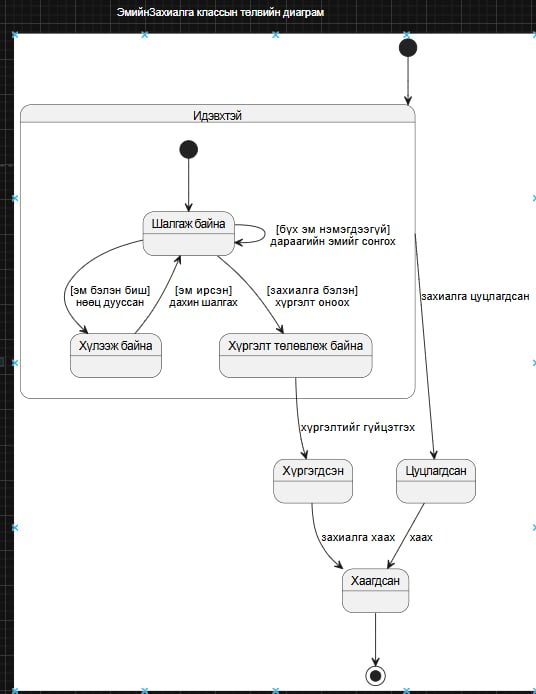
\includegraphics[width=9cm]{Diagrams/state_pharmacy.PNG}
    \caption[Эмийн захиалгын төлвийн диаграм]{Эмийн захиалгын төлвийн диаграм}
    \begin{itemize}
        \item \textbf{Эхлэл:} Процесс нь \textit{Захиалга үүсгэх} үе шатнаас эхэлнэ.
        
        \item \textbf{Дотоод үйл явц:}
        \begin{itemize}
            \item \textbf{Захиалгын дэлгэрэнгүй мэдээлэл оруулах:} Захиалгын эм, тоо хэмжээ, хэрэглэгчийн мэдээллийг бүртгэнэ.
            \item \textbf{Аптек/Ажилтанд хуваарилах:} Захиалга боловсруулагдаж ажилтанд хуваарилагдана.
            \item \textbf{Захиалгыг шалгах:} Ажилтан захиалгыг гүйцэтгэж дууссаныг хянаж баталгаажуулна.
            \item \textbf{Батлах эсвэл Засварлах:}
            \begin{itemize}
                \item \textbf{Батлах:} Захиалга зөвшөөрөгдсөн бол батлагдана.
                \item \textbf{Засварлах:} Алдаа гарвал засварлаж, дахин шалгана.
            \end{itemize}
        \end{itemize}
        
        \item \textbf{Захиалгыг дуусгах:} Захиалга зөвшөөрөгдсөн тохиолдолд “Дууссан” төлөвт шилжинэ.
        
        \item \textbf{Төгсгөл:} Процесс \textit{Closed} төлөвт хүрч дуусна.
    \end{itemize}
\end{figure}

    

%-----------------------------------------------------------------------
    
\section{Дэлгэцийн зохиомж}
\begin{figure}[H]
	\centering
	\includegraphics[width=13cm,heigth=12cm]{Diagrams/login.PNG}
	\caption[Нэвтрэх дэлгэц]{Нэвтрэх дэлгэц}
\end{figure}
\subsection{Бүртгүүлэх хэсэг}
\begin{figure}[H]
	\centering
	\includegraphics[width=13cm,heigth=12cm]{Diagrams/register.PNG}
	\caption[Бүртгэлийн дэлгэц]{Бүртгэлийн дэлгэц}
\end{figure}

\end{figure}
